\documentclass[conference]{IEEEtran}

\usepackage[utf8]{inputenc}
\usepackage[T1]{fontenc}
\usepackage[spanish,es-tabla,es-noshorthands]{babel}
\usepackage{cite}
\usepackage{amsmath,amssymb,amsfonts}
\usepackage{graphicx}
\usepackage{booktabs}
\usepackage{multirow}
\usepackage{array}
\usepackage{float}
\usepackage{tikz}
\usetikzlibrary{arrows.meta,positioning,shapes.geometric}
\usepackage[hyphens]{url}
\usepackage[hidelinks]{hyperref}

% Adaptación de encabezados IEEEtran al español
\addto\captionsspanish{%
  \renewcommand{\abstractname}{Resumen}%
  \renewcommand{\IEEEkeywordsname}{Palabras clave}%
  \renewcommand{\refname}{Referencias}%
}

\hyphenation{pre-pro-ce-sa-mien-to hi-per-pa-rá-me-tros cla-si-fi-ca-ción es-tra-ti-fi-ca-da}

\begin{document}

\title{Evaluación Experimental y Optimización de Modelos de Aprendizaje Automático para la Predicción de Riesgo e Incumplimiento Crediticio}

\author{%
\IEEEauthorblockN{Joel Arturo Álvarez Hernández}
\IEEEauthorblockA{%
Facultad de Ingeniería, Maestría en Machine Learning\\
Universidad Autónoma de Chihuahua (UACH)\\
Matrícula: 403233 --- Asesora: Dra. Olanda Prieto Ordaz\\
Chihuahua, México}
}

\maketitle

\begin{abstract}
La evaluación del riesgo crediticio representa un problema de clasificación binaria crítico por el costo asimétrico entre aprobar créditos con incumplimiento y rechazar solicitantes solventes. El objetivo de este trabajo es diseñar, optimizar y evaluar experimentalmente un flujo de aprendizaje automático libre de fuga de información para priorizar la detección de incumplimientos (\texttt{loan\_status=1}). Utilizando el \textit{Credit Risk Dataset} de Kaggle ($32{,}581$ instancias y $12$ atributos), se aplicó limpieza determinista ($28{,}495$ registros válidos tras eliminar $165$ duplicados, $3{,}915$ filas con valores vacíos y $6$ atípicos imposibles), partición estratificada $80/20$ ($22{,}796$ entrenamiento; $5{,}699$ prueba) y validación cruzada estratificada de $5$ pliegues dentro de arquitecturas \textit{Pipeline} y \textit{ColumnTransformer} con estandarización numérica y codificación \textit{One-Hot}. Se evaluaron Regresión Logística, Máquinas de Vectores de Soporte con kernel RBF (\textit{SVM RBF}) y \textit{Random Forest}, optimizando hiperparámetros y umbrales de decisión en entrenamiento bajo la métrica $F_2$ (ponderando la exhaustividad $2\times$ sobre la precisión). Bajo $F_2$, los tres modelos seleccionaron \texttt{class\_weight="balanced"} y \textit{Random Forest} obtuvo el mejor desempeño en prueba ($\text{Recall}=0.7898$, $F_2=0.7977$, $F_1=0.8098$, $\text{ROC-AUC}=0.9381$) en $0.55\text{ s}$, confirmando que los ensambles de árboles capturan con superior eficacia las relaciones no lineales del riesgo crediticio.
\end{abstract}

% =========================================================================
\section{Introducción}
% =========================================================================

La creacion de un crédito y la evaluación del riesgo de incumplimiento representan procesos de suma importancia dentro del sector bancario y de tecnología financiera (\textit{FinTech}). La decisión de otorgar o denegar un préstamo ha dependido de reglas rígidas, comités manuales de análisis y puntuaciones estadísticas tradicionales que resultan lentas para operar a escala. En un entorno caracterizado por volúmenes crecientes de solicitudes digitales y por márgenes estrechos entre rentabilidad y morosidad, automatizar la detección temprana de riesgo mediante herramientas objetivas constituye una necesidad operativa estratégica~\cite{pucar2026consumer,lin2026automl}.

El problema técnico abordado consiste en la clasificación binaria supervisada de solicitudes de préstamo a partir de atributos demográficos, laborales, financieros, calificación crediticia de la operación e historial en buró del solicitante. Desde la perspectiva financiera, la tarea conlleva una cantidad de costos considerable: aprobar una operación que deriva en incumplimiento (falso negativo respecto a \texttt{loan\_status=1}) acarrea pérdidas directas de capital e intereses, mientras que clasificar erróneamente a un solicitante solvente como riesgoso (falso positivo) implica pérdida de ingresos comerciales y deterioro en la retención de clientes~\cite{pucar2026consumer}. Además, las bases de datos crediticias reales presentan valores vacíos o faltantes, duplicados, registros atípicos de captura, desbalance natural de clases, correlaciones entre edad e historial crediticio, y codificaciones categóricas heterogéneas que condicionan fuertemente la estabilidad del aprendizaje~\cite{maurino2025dataquality,bolikulov2024categorical}.

Para enfrentar estos retos, las soluciones computacionales modernas han utilizado desde modelos lineales generalizados como la Regresión Logística~\cite{cox1958regression} hasta clasificadores basados en márgenes no lineales como las Máquinas de Vectores de Soporte (\textit{Support Vector Machines}, SVM)~\cite{cortes1995support}, métodos de ensamble basados en árboles como \textit{Random Forest}~\cite{breiman2001random} y \textit{Gradient Boosting}~\cite{pucar2026consumer}, plataformas de aprendizaje automatizado (\textit{AutoML})~\cite{lin2026automl} y ensambles de apilamiento optimizados bayesianamente~\cite{mahmud2025stacking}. Si bien múltiples estudios reportan métricas prometedoras, un desafío metodológico recurrente radica en garantizar una depuración rigurosa de calidad de datos y la ausencia de fuga de información (\textit{data leakage}) durante el filtrado de duplicados, valores vacíos, atípicos, codificación categórica y búsqueda de hiperparámetros~\cite{maurino2025dataquality,bolikulov2024categorical}.

El objetivo principal de este proyecto es desarrollar, optimizar y evaluar experimentalmente un sistema modular de aprendizaje automático en Python para predecir el incumplimiento crediticio sobre la base de datos pública \textit{Credit Risk Dataset}~\cite{laotse_credit_risk}, contrastando tres familias algorítmicas representativas: Regresión Logística (modelo lineal interpretable), SVM con kernel RBF (clasificador geométrico no lineal) y \textit{Random Forest} (ensamble paralelo de árboles de decisión). Dado el mayor costo financiero de omitir casos de incumplimiento (clase $1$), la optimización de hiperparámetros y de umbrales de decisión en validación cruzada se orientó mediante el puntaje $F_2$. El alcance del trabajo comprende el análisis exploratorio y depuración determinista del conjunto de $32{,}581$ registros brutos ($28{,}495$ válidos completos), el diseño de un flujo encapsulado libre de fuga de datos mediante \texttt{scikit-learn}~\cite{pedregosa2011scikit}, la evaluación \textit{baseline} y optimizada en validación cruzada estratificada de $5$ pliegues en entrenamiento (incluyendo mapas 2D $F_2$, curvas 1D y ajuste de umbral en CV), la evaluación final en un conjunto de prueba independiente, el contraste con cinco investigaciones del estado del arte y la publicación del código reproducible y aplicación web en Streamlit.\footnote{Código fuente y artefactos experimentales disponibles en \url{https://github.com/MrAkuDev/loan_approval}.}

% =========================================================================
\section{Antecedentes y Trabajos Relacionados}
% =========================================================================

La literatura reciente sobre riesgo crediticio contiene cinco referencias directamente relacionados con este proyecto: impacto de la calidad de datos, desempeño de ensambles, plataformas \textit{AutoML}, codificación de variables categóricas y apilamiento optimizado. A continuación se referencian cinco estudios representativos y se resumen sus modelos y métricas en la Tabla~\ref{tab:antecedentes_modelos}.

\begin{itemize}
\item \textbf{Calidad de datos (\textit{Data-Centric AI}):} Maurino~\cite{maurino2025dataquality} evaluó mediante \textit{Pucktrick} cómo valores faltantes, ruido, atípicos y errores de etiqueta degradan clasificadores en un conjunto abierto de riesgo crediticio. Sobre el dataset limpio reportó como referencia base $9$ modelos (Tabla~\ref{tab:antecedentes_modelos}).
\item \textbf{Ensambles en banca minorista:} Pucar y Soleša~\cite{pucar2026consumer} compararon Regresión Logística, \textit{Random Forest} y \textit{Gradient Boosting}, evidenciando la brecha de exhaustividad frente al modelo lineal y el peso dominante de la calificación crediticia, tasa de interés y razón préstamo-ingreso.
\item \textbf{Comparativa AutoML:} Lin~\cite{lin2026automl} evaluó \textit{H2O AutoML}, \textit{Azure AutoML} y \textit{TPOT} frente a Regresión Logística en predicción de incumplimiento. \textit{H2O AutoML} y \textit{Azure AutoML} alcanzaron el mejor balance ($\text{AUC}=0.918$ y $0.917$; $F_1=0.724$ y $0.718$), mientras que \textit{TPOT} maximizó la precisión ($0.948$) sacrificando exhaustividad ($0.524$).
\item \textbf{Codificación categórica:} Bolikulov \textit{et al.}~\cite{bolikulov2024categorical} contrastaron $14$ técnicas (\textit{One-Hot}, \textit{Target}, \textit{Binary}, \textit{Gray}, ordinal, \textit{CatBoost}, \textit{Label}) sobre riesgo crediticio real evaluado con un clasificador logístico, demostrando que codificaciones sin sesgo ordinal artificial evitan degradaciones severas en $F_1$ ($0.5645$ con \textit{Gray} frente a $\approx 0.38$ con \textit{Label Encoding}) y que \textit{One-Hot Encoding} es esencial para modelos lineales y geométricos.
\item \textbf{Apilamiento bayesiano (\textit{BO-StaEnsemble}):} Mahmud \textit{et al.}~\cite{mahmud2025stacking} compararon $9$ clasificadores base (\textit{Decision Tree}, \textit{Logistic Regression}, \textit{Random Forest}, \textit{K-Nearest Neighbors}, \textit{AdaBoost}, \textit{Gradient Boosting}, \textit{XGBoost}, \textit{LightGBM} y \textit{CatBoost}) frente a su ensamble \textit{BO-StaEnsemble} (Optuna + meta-clasificador logístico + ADASYN) sobre el \textit{Credit Risk Dataset}, logrando $\text{Accuracy}=0.9600$, especificidad (\textit{Precision}) $=0.9822$, sensibilidad (\textit{Recall}) $=0.9323$, $\text{MCC}=0.9159$, $\kappa=0.9147$ y $\text{ROC-AUC}=0.998$ ($p < 0.001$), con explicabilidad SHAP/LIME.
\end{itemize}

\begin{table*}[t]
\centering
\footnotesize
\setlength{\tabcolsep}{7pt}
\caption{Métricas de Desempeño de Modelos en los Trabajos Relacionados (incluyendo el baseline limpio de Maurino~\cite{maurino2025dataquality})}
\label{tab:antecedentes_modelos}
\begin{tabular}{@{}llcccc@{}}
\toprule
\textbf{Referencia} & \textbf{Model} & \textbf{Accuracy} & \textbf{Precision} & \textbf{Recall} & \textbf{F1\_Score} \\
\midrule
\multirow{9}{*}{Maurino (2025)~\cite{maurino2025dataquality} (dataset limpio)} & Linear Discriminant Analysis & \textbf{0.9354} & \textbf{0.9690} & 0.7192 & \textbf{0.8256} \\
& Extra Trees & 0.8821 & 0.7129 & \textbf{0.7463} & 0.7292 \\
& Logistic Regression & 0.9219 & 0.9011 & 0.7110 & 0.7949 \\
& Random Forest & 0.8680 & 0.7296 & 0.6026 & 0.6601 \\
& K-Nearest Neighbors & 0.8533 & 0.7345 & 0.4860 & 0.5850 \\
& Multi-Layer Perceptron & 0.8551 & 0.6535 & 0.6782 & 0.6656 \\
& Naive Bayes & 0.8247 & 0.7131 & 0.2939 & 0.4163 \\
& Decision Tree & 0.8200 & 0.7221 & 0.2496 & 0.3710 \\
& Support Vector Machine & 0.7997 & 0.7290 & 0.0928 & 0.1646 \\
\midrule
\multirow{3}{*}{Pucar y Soleša (2026)~\cite{pucar2026consumer}$^{\mathrm{a}}$} & Gradient Boosting & \textbf{0.934} & 0.958 & \textbf{0.732} & \textbf{0.830} \\
& Random Forest & 0.926 & \textbf{0.961} & 0.690 & 0.803 \\
& Logistic Regression & 0.843 & 0.713 & 0.470 & 0.566 \\
\midrule
\multirow{3}{*}{Lin (2026)~\cite{lin2026automl}$^{\mathrm{b}}$} & H2O AutoML & \textbf{0.9020} & --- & --- & \textbf{0.7240} \\
& Azure AutoML & 0.8990 & --- & --- & 0.7180 \\
& Tree-based Pipeline Optimization Tool (TPOT) & --- & \textbf{0.9480} & \textbf{0.5240} & --- \\
\midrule
\multirow{2}{*}{Bolikulov \textit{et al.} (2024)~\cite{bolikulov2024categorical}} & Logistic Regression + Gray Coding & \textbf{0.8203} & \textbf{0.4454} & \textbf{0.7704} & \textbf{0.5645} \\
& Logistic Regression + Label Encoding & 0.7719 & 0.2701 & 0.6551 & $\approx 0.38$ \\
\midrule
\multirow{10}{*}{Mahmud \textit{et al.} (2025)~\cite{mahmud2025stacking}$^{\mathrm{c}}$} & Decision Tree & 0.8770 & 0.8721 & 0.8820 & 0.8770 \\
& Logistic Regression & 0.7031 & 0.7127 & 0.6933 & 0.7030 \\
& Random Forest & 0.9454 & 0.9588 & 0.9318 & 0.9453 \\
& K-Nearest Neighbors & 0.8597 & 0.7406 & \textbf{0.9804} & 0.8605 \\
& AdaBoost & 0.7840 & 0.8043 & 0.7635 & 0.7839 \\
& Gradient Boosting & 0.8749 & 0.9173 & 0.8319 & 0.8746 \\
& XGBoost & 0.9484 & 0.9862 & 0.9102 & 0.9482 \\
& LightGBM & 0.9477 & 0.9920 & 0.9030 & 0.9475 \\
& CatBoost & 0.9534 & \textbf{0.9955} & 0.9106 & 0.9530 \\
& \textbf{BO-StaEnsemble} & \textbf{0.9600} & 0.9822 & 0.9323 & \textbf{0.9572} \\
\bottomrule
\multicolumn{6}{@{}p{13.8cm}@{}}{\scriptsize $^{\mathrm{a}}$AUC-ROC reportado: Gradient Boosting $0.950$, Random Forest $0.927$, Logistic Regression $0.845$. $^{\mathrm{b}}$ROC-AUC reportado: H2O $0.918$, Azure $0.917$. $^{\mathrm{c}}$En Mahmud \textit{et al.}~\cite{mahmud2025stacking} se homologan \textit{Specificity} $\rightarrow$ \textit{Precision}, \textit{Sensitivity} $\rightarrow$ \textit{Recall} y \textit{F1\_Score} $= (\text{Recall}+\text{Precision})/2$ ($\text{MCC}=0.9159$, $\kappa=0.9147$ para \textit{BO-StaEnsemble}).}
\end{tabular}
\end{table*}

El proyecto toma estas aportaciones sobre \textit{Credit Risk Dataset}~\cite{laotse_credit_risk} eliminando primero duplicados exactos, filas vacías (preservando el cero numérico válido) y atípicos imposibles~\cite{maurino2025dataquality}, aplicando \texttt{OneHotEncoder}~\cite{bolikulov2024categorical} y escalamiento dentro de \texttt{Pipeline}, y comparando Regresión Logística, \textit{SVM RBF} y \textit{Random Forest}.

% =========================================================================
\section{Metodología}
% =========================================================================

La metodología se implementó dentro del paquete principal \texttt{model\_factory}, diseñado para asegurar separación estricta entre entrenamiento y prueba, trazabilidad de semillas aleatorias y persistencia de artefactos reproducibles consumidos posteriormente por la aplicación web en Streamlit.

\subsection{Descripción de la Base de Datos}

El estudio emplea la base de datos pública \textit{Credit Risk Dataset} (\texttt{credit\_risk\_dataset.csv}), disponible en Kaggle~\cite{laotse_credit_risk}. Su propósito original es simular y modelar el riesgo de incumplimiento de préstamos personales a partir de características demográficas, estabilidad laboral, nivel de ingresos, condiciones financieras del crédito, calificación interna (\texttt{loan\_grade}) e historial previo en buró. En su forma original, el archivo contiene $=32{,}581$ instancias y $12$ caracteristicas ($11$ variables predictoras y $1$ variable objetivo binaria \texttt{loan\_status}), con $165$ filas duplicadas exactas, $3{,}915$ filas con celdas vacías en \texttt{person\_emp\_length} o \texttt{loan\_int\_rate} y $6$ registros físicamente imposibles restantes.

Tras una depuración determinista previa a la partición —que conserva $28{,}495$ instancias completas y válidas ($0$ valores vacíos)—, las $11$ variables predictoras se dividen en $7$ atributos numéricos y $4$ atributos categóricos. La Tabla~\ref{tab:dataset_schema} detalla el esquema completo de variables, su tipo, dominio válido y estadísticos descriptivos sobre los $28{,}495$ registros limpios.

\begin{table*}[t]
\centering
\scriptsize
\setlength{\tabcolsep}{4pt}
\caption{Esquema y Estadísticos Descriptivos de \texttt{credit\_risk\_dataset.csv} ($N=28{,}495$ limpios; $32{,}581$ brutos)}
\label{tab:dataset_schema}
\begin{tabular}{@{}llp{2.25cm}p{4.65cm}p{4.45cm}@{}}
\toprule
\textbf{Variable} & \textbf{Tipo} & \textbf{Rango / Dominio} & \textbf{Resumen Estadístico / Frecuencia} & \textbf{Descripción Técnica} \\
\midrule
\texttt{person\_age} & Numérica & $20 - 84$ ($0$ vacíos) & Media: $27.72 \pm 6.18$ (Mediana: $26$) & Edad del solicitante en años (se filtraron casos $>100$: $123$ y $144$). \\
\texttt{person\_income} & Numérica & $\$4{,}000 - \$2{,}039{,}784$ & Media: $\$66{,}430 \pm \$51{,}514$ (Med.: $\$56{,}000$) & Ingreso anual declarado en USD. Distribución asimétrica positiva. \\
\texttt{person\_emp\_length} & Numérica & $0.0 - 41.0$ ($0$ vacíos) & Media: $4.78 \pm 4.04$ (Mediana: $4.0$) & Antigüedad laboral en años ($0$ válido; se excluyeron $887$ vacíos y casos de $123$ años). \\
\texttt{loan\_amnt} & Numérica & $\$500 - \$35{,}000$ ($0$ vacíos) & Media: $\$9{,}657 \pm \$6{,}328$ (Med.: $\$8{,}000$) & Monto principal del préstamo solicitado (USD). \\
\texttt{loan\_int\_rate} & Numérica & $5.42\% - 23.22\%$ ($0$ vacíos) & Media: $11.05\% \pm 3.23\%$ (Med.: $10.99\%$) & Tasa de interés anual asignada (se excluyeron $3{,}095$ filas vacías). \\
\texttt{loan\_percent\_income} & Numérica & $0.00 - 0.83$ ($0$ vacíos) & Media: $0.17 \pm 0.11$ (Mediana: $0.15$) & Razón entre monto solicitado e ingreso anual (\texttt{loan\_amnt / person\_income}). \\
\texttt{cb\_person\_cred\_hist\_length} & Numérica & $2 - 30$ ($0$ vacíos) & Media: $5.80 \pm 4.04$ (Mediana: $4$) & Antigüedad del historial crediticio en el buró (años). \\
\midrule
\texttt{person\_home\_ownership} & Categórica & 4 categorías & \texttt{RENT} ($14{,}495$), \texttt{MORTGAGE} ($11{,}733$), \texttt{OWN} ($2{,}174$), \texttt{OTHER} ($93$) & Situación de tenencia de vivienda del solicitante. \\
\texttt{loan\_intent} & Categórica & 6 categorías & \texttt{EDUCATION} ($5{,}668$), \texttt{MEDICAL} ($5{,}269$), \texttt{VENTURE} ($4{,}967$), \texttt{PERSONAL} ($4{,}857$), \texttt{DEBTCONSOLIDATION} ($4{,}547$), \texttt{HOMEIMPROVEMENT} ($3{,}187$) & Propósito financiero declarado del crédito solicitado. \\
\texttt{loan\_grade} & Categórica & 7 categorías & \texttt{A} ($9{,}344$), \texttt{B} ($9{,}092$), \texttt{C} ($5{,}680$), \texttt{D} ($3{,}242$), \texttt{E} ($869$), \texttt{F} ($209$), \texttt{G} ($59$) & Grado de riesgo asignado al préstamo (\texttt{A}: menor riesgo a \texttt{G}: mayor riesgo). \\
\texttt{cb\_person\_default\_on\_file} & Categórica & 2 categorías & \texttt{N} ($23{,}406$), \texttt{Y} ($5{,}089$) & Registro histórico binario de incumplimientos previos en buró. \\
\midrule
\texttt{loan\_status} & Objetivo & $\{0, 1\}$ & \texttt{0}: $22{,}308$ ($78.29\%$), \texttt{1}: $6{,}187$ ($21.71\%$) & Estado del crédito ($0$: Sin Incumplimiento, $1$: Incumplimiento). \\
\bottomrule
\end{tabular}
\end{table*}

La variable objetivo binaria \texttt{loan\_status} presenta un desbalance moderado de $3.61:1$, compuesto por $22{,}308$ instancias de clase negativa (\textbf{Sin Incumplimiento (0)}, $78.29\%$) y $6{,}187$ de clase positiva (\textbf{Incumplimiento (1)}, $21.71\%$), mostrado en la Fig.~\ref{fig:dataset_eda}(a). El análisis exploratorio revela patrones de riesgo financieramente consistentes y altamente informativos. En primer lugar, la calificacion crediticia \texttt{loan\_grade} exhibe una progresión monótona con una discontinuidad abrupta entre los grados \texttt{C} y \texttt{D}: mientras los grados \texttt{A}, \texttt{B} y \texttt{C} presentan tasas de incumplimiento de $9.61\%$, $15.93\%$ y $20.33\%$, la tasa salta a $59.22\%$ en \texttt{D}, $64.67\%$ en \texttt{E}, $69.86\%$ en \texttt{F} y $98.31\%$ en \texttt{G} (Fig.~\ref{fig:dataset_eda}(b)). En segundo lugar, quienes registran mora previa en buró (\texttt{cb\_person\_default\_on\_file="Y"}) duplican la tasa de incumplimiento ($37.83\%$ vs.\ $18.21\%$ en \texttt{"N"}), y quienes rentan vivienda (\texttt{RENT}) alcanzan $31.27\%$ de incumplimiento frente a $12.64\%$ en hipoteca (\texttt{MORTGAGE}) y $6.67\%$ en vivienda propia (\texttt{OWN}). En promedio, los casos de incumplimiento (\texttt{loan\_status=1}) exhiben menor ingreso anual ($\$50{,}017$ vs.\ $\$70{,}983$), mayor razón préstamo-ingreso ($0.2462$ vs.\ $0.1482$) y tasas de interés superiores ($13.13\%$ vs.\ $10.47\%$).

\begin{figure*}[t]
\centering
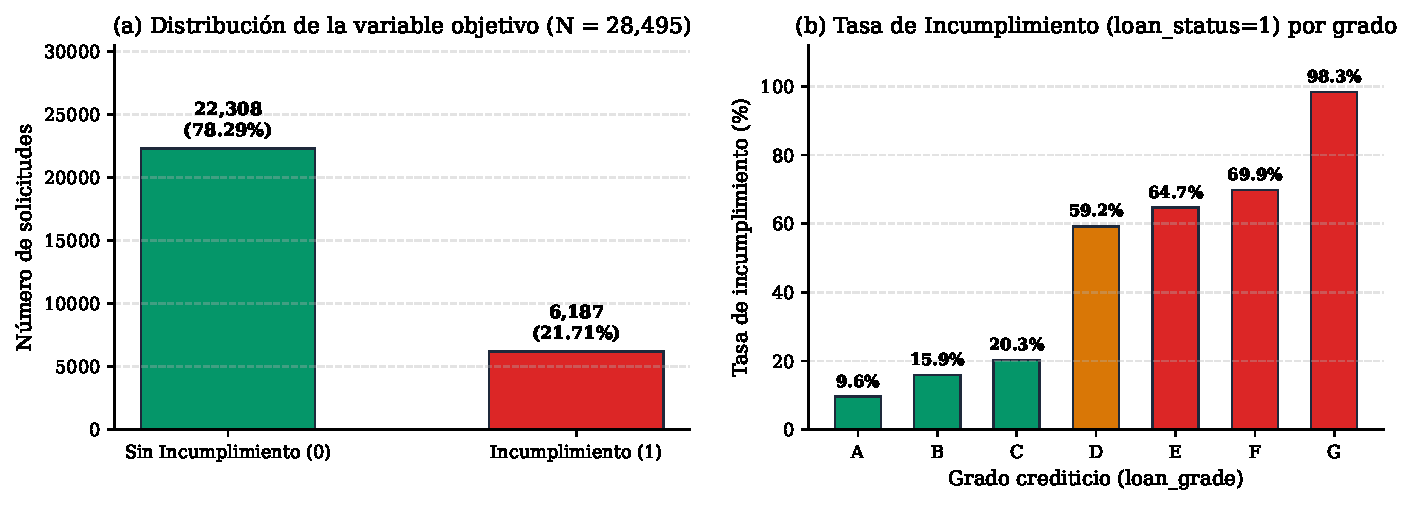
\includegraphics[width=0.92\textwidth]{figures/fig1_dataset_eda.pdf}
\caption{Análisis exploratorio de \texttt{credit\_risk\_dataset.csv} tras limpieza determinista ($N=28{,}495$): (a) distribución desbalanceada de \texttt{loan\_status} ($78.29\%$ Sin Incumplimiento (0) vs.\ $21.71\%$ Incumplimiento (1)); (b) tasa empírica de incumplimiento (\texttt{loan\_status=1}) según el grado crediticio \texttt{loan\_grade}, evidenciando el salto crítico a partir del grado \texttt{D} ($59.22\%$) hasta \texttt{G} ($98.31\%$).}
\label{fig:dataset_eda}
\end{figure*}

\subsection{Análisis Exploratorio y Preprocesamiento}

Para garantizar validez estadística e impedir cualquier fuga de información hacia la validación cruzada o el conjunto de prueba, la limpieza determinista se separó estrictamente de las transformaciones paramétricas: únicamente las reglas independientes de la muestra completa se ejecutaron antes de \texttt{train\_test\_split}, mientras que toda estimación estadística (imputación, media, desviación estándar y categorías) quedó encapsulada dentro del paso \texttt{"preprocesamiento"} (\texttt{ColumnTransformer}) del \texttt{Pipeline} de \texttt{scikit-learn}~\cite{pedregosa2011scikit}, ajustado exclusivamente sobre $X_{\text{train}}$. Las decisiones aplicadas fueron:

\begin{itemize}
\item \textbf{Deduplicación exacta:} La auditoría del archivo bruto ($32{,}581$ filas) detectó $165$ registros duplicados exactos. Su eliminación previa a la partición ($32{,}416$ filas restantes) es indispensable para evitar que copias idénticas aparezcan simultáneamente en entrenamiento y prueba, inflando artificialmente la generalización por memorización.
\item \textbf{Exclusión de registros con valores vacíos:} Al exigir que las $12$ columnas contengan información válida (distinguiendo celdas vacías/\texttt{NaN} del valor numérico $0$, como $0.0$ años de antigüedad laboral), se excluyeron $3{,}915$ registros incompletos ($887$ vacíos en \texttt{person\_emp\_length} y $3{,}095$ en \texttt{loan\_int\_rate}, con $67$ coincidentes), quedando $28{,}501$ observaciones íntegras sin necesidad de imputación sintética.
\item \textbf{Filtrado de valores físicamente imposibles:} Sobre las filas completas se detectaron $6$ registros incompatibles con la realidad ($4$ solicitantes con \texttt{person\_age} igual a $123$ o $144$ años y $2$ solicitantes con \texttt{person\_emp\_length} de $123.0$ años). Aplicando los umbrales deterministas \texttt{person\_age <= 100} y \texttt{person\_emp\_length <= 60}, se obtuvo el conjunto limpio de $N=28{,}495$ registros con $0$ valores vacíos. Las colas plausibles de ingreso (hasta $\$2{,}039{,}784$) se conservaron intactas.
\item \textbf{Escalamiento numérico:} Siguiendo el principio de encapsular transformaciones únicamente sobre los datos de entrenamiento para evitar fuga de información~\cite{muller2016introduction}, las $7$ variables numéricas se transforman dentro del \texttt{ColumnTransformer} mediante estandarización $z$-score (\texttt{StandardScaler}, precedida de \texttt{SimpleImputer} como respaldo defensivo en inferencia). Como detallan Müller y Guido~\cite{muller2016introduction}, escalar a media cero y varianza unitaria es crítico para algoritmos sensibles a escala como \textit{SVM RBF} y modelos lineales regularizados.
\item \textbf{Codificación categórica:} Las $4$ variables categóricas nominales se representan mediante \texttt{OneHotEncoder} con \texttt{drop="first"}, \texttt{handle\_unknown="ignore"} y \texttt{sparse\_output=False}~\cite{muller2016introduction,bolikulov2024categorical}, generando variables indicadoras binarias sin asumir orden numérico artificial y conformando junto con las $7$ numéricas un espacio unificado de $22$ características procesadas ($7$ numéricas $+$ $15$ binarias \textit{dummy}).
\item \textbf{Análisis de correlaciones:} La matriz de correlación de Pearson se calculó exclusivamente sobre $X_{\text{train}}$ ($22{,}796$ muestras) tras codificación \textit{dummy} con \texttt{drop\_first=True}. Como muestra la Fig.~\ref{fig:correlaciones}, las asociaciones lineales positivas más fuertes con el riesgo de incumplimiento (\texttt{loan\_status=1}) corresponden a \texttt{loan\_percent\_income} ($r=+0.3754$), \texttt{loan\_int\_rate} ($r=+0.3394$), \texttt{loan\_grade\_D} ($r=+0.3288$), \texttt{person\_home\_ownership\_RENT} ($r=+0.2375$), \texttt{loan\_grade\_E} ($r=+0.1846$) y \texttt{cb\_person\_default\_on\_file\_Y} ($r=+0.1814$), mientras que las correlaciones negativas protectoras más marcadas recaen en \texttt{person\_income} ($r=-0.1653$) y \texttt{person\_home\_ownership\_OWN} ($r=-0.1064$). Entre predictores numéricos destaca la colinealidad esperada entre \texttt{person\_age} y \texttt{cb\_person\_cred\_hist\_length} ($r=0.8767$).
\item \textbf{Selección de características y manejo del desbalance:} Con $22$ dimensiones finales y $22{,}796$ muestras de entrenamiento (razón $>1{,}036$ muestras por dimensión), se retuvieron los $11$ atributos originales sin reducción PCA para preservar interpretabilidad y no destruir interacciones no lineales entre tasa, grado y propósito. Para abordar el desbalance $78.29\% / 21.71\%$ sin distorsionar probabilidades calibradas mediante SMOTE, se evaluó \texttt{class\_weight} $\in \{\texttt{None}, \texttt{"balanced"}\}$ directamente en la búsqueda de hiperparámetros bajo CV.
\end{itemize}

\begin{figure}[t]
\centering
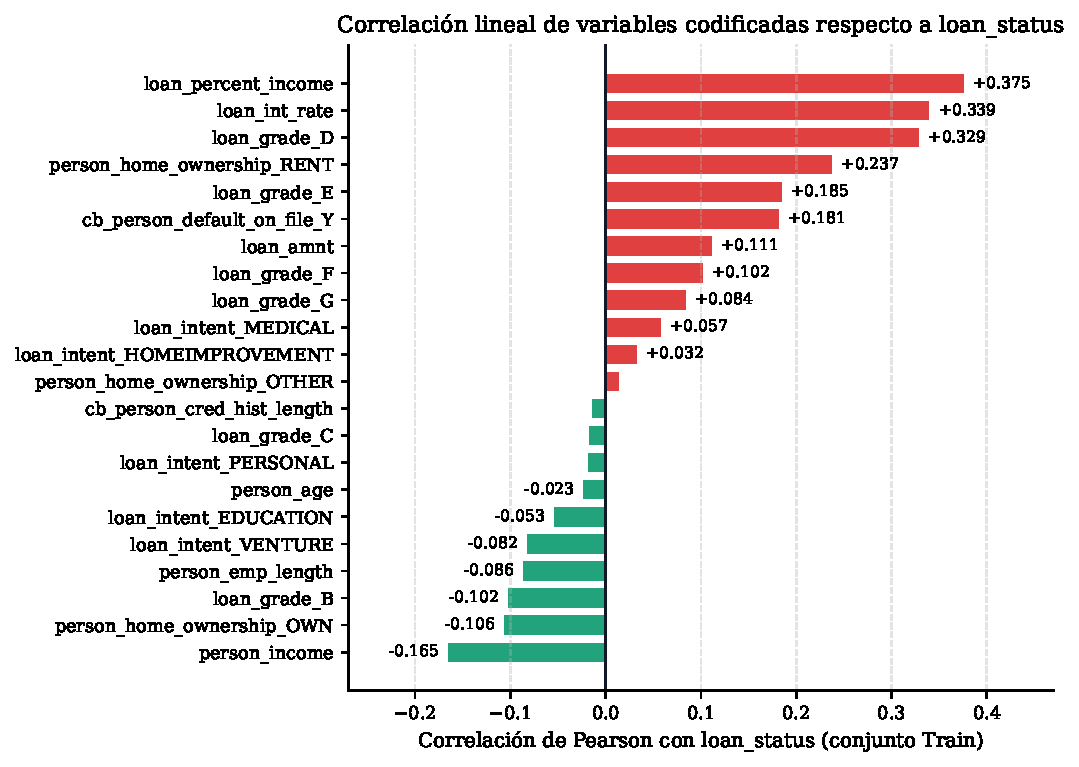
\includegraphics[width=\columnwidth]{figures/fig2_correlaciones.pdf}
\caption{Correlaciones lineales de Pearson calculadas exclusivamente sobre $X_{\text{train}}$ ($22{,}796$ muestras) respecto a \texttt{loan\_status} (Incumplimiento (1)). Destacan \texttt{loan\_percent\_income} ($+0.3754$), \texttt{loan\_int\_rate} ($+0.3394$) y \texttt{loan\_grade\_D} ($+0.3288$) como factores de riesgo, frente a \texttt{person\_income} ($-0.1653$) y vivienda propia ($-0.1064$) como factores protectores.}
\label{fig:correlaciones}
\end{figure}

\subsection{Modelos de Machine Learning}

Se seleccionaron tres clasificadores supervisados para contrastar fronteras lineales, separadores no lineales basados en núcleo y particionamiento jerárquico por ensamble:

\subsubsection{Regresión Logística}
La Regresión Logística~\cite{cox1958regression,muller2016introduction} modela directamente la probabilidad posterior de incumplimiento mediante la función sigmoide~\eqref{eq:logreg} aplicada a una combinación lineal de los atributos procesados $\mathbf{x} \in \mathbb{R}^{22}$:
\begin{equation}
P(y = 1 \mid \mathbf{x}) = \sigma(\mathbf{w}^\top \mathbf{x} + b) = \frac{1}{1 + \exp\big(-(\mathbf{w}^\top \mathbf{x} + b)\big)},
\label{eq:logreg}
\end{equation}
estimando $(\mathbf{w}, b)$ mediante minimización de la entropía cruzada binaria con regularización $L_2$ controlada por el parámetro inverso $C$, donde valores menores de $C$ penalizan los coeficientes hacia cero buscando mayor simplicidad y valores mayores permiten ajustar más fielmente los datos de entrenamiento~\cite{muller2016introduction}. Fue elegida como referencia paramétrica lineal por su eficiencia ($<0.4\text{ s}$), calibración probabilística nativa e interpretabilidad directa de pesos, empleando el optimizador \texttt{lbfgs} con \texttt{max\_iter=1000}.

\subsubsection{Máquina de Vectores de Soporte con Kernel RBF (SVM RBF)}
Las SVM~\cite{cortes1995support,muller2016introduction} buscan el hiperplano separador de margen máximo entre clases empleando el truco del núcleo (\textit{kernel trick}) gaussiano o de Función de Base Radial (RBF) definido en~\eqref{eq:svm_rbf}:
\begin{equation}
K(\mathbf{x}_i, \mathbf{x}_j) = \exp\big(-\gamma \|\mathbf{x}_i - \mathbf{x}_j\|^2\big), \quad \gamma > 0,
\label{eq:svm_rbf}
\end{equation}
donde $\gamma$ regula el alcance de influencia de cada vector de soporte (ancho del núcleo gaussiano) y $C$ limita la importancia permitida a cada instancia individual~\cite{muller2016introduction}. Debido a su sensibilidad a la escala euclidiana de los atributos, se integró estrictamente tras \texttt{StandardScaler} para evaluar fronteras suaves no lineales. Para agilizar la validación cruzada y búsqueda de hiperparámetros, el escalado de Platt (\texttt{probability=True}) se activó únicamente durante el entrenamiento final vía \texttt{final\_extra\_params}.

\subsubsection{Random Forest}
\textit{Random Forest}~\cite{breiman2001random,muller2016introduction} construye un ensamble paralelo de $B$ (\texttt{n\_estimators}) árboles de decisión sin podado entrenados sobre muestras \textit{bootstrap} distintas, inyectando aleatoriedad adicional al evaluar en cada nodo solo un subconjunto de $m$ variables (\texttt{max\_features}) para decorrelacionar los árboles y reducir el sobreajuste~\cite{muller2016introduction}. Cada partición optimiza la reducción de la impureza de Gini~\eqref{eq:gini}:
\begin{equation}
G(t) = 1 - \sum_{k \in \{0,1\}} p_{t,k}^2,
\label{eq:gini}
\end{equation}
donde $p_{t,k}$ representa la proporción de la clase $k$ en el nodo $t$, promediando posteriormente las probabilidades estimadas entre los $B$ árboles. Se seleccionó por su desempeño sobresaliente en la literatura crediticia~\cite{pucar2026consumer,maurino2025dataquality,mahmud2025stacking}, su invarianza ante escalamiento monótono y su tolerancia a saltos abruptos entre categorías como \texttt{loan\_grade} \texttt{C} y \texttt{D}, ejecutándose en paralelo con \texttt{n\_jobs=-1}.

\subsection{Configuración Experimental}

La investigacion consta de tres etapas secuenciales ejecutadas por \texttt{model\_factory/train\_model.py}, ilustradas en la Fig.~\ref{fig:methodology_diagram}.

\begin{figure*}[t]
\centering
\begin{tikzpicture}[
    node distance=0.45cm and 0.55cm,
    box/.style={rectangle, rounded corners=3pt, draw=black!75, fill=blue!6, thick, minimum height=1.1cm, text width=3.55cm, align=center, font=\footnotesize},
    stage/.style={rectangle, rounded corners=3pt, draw=teal!80!black, fill=teal!7, thick, minimum height=1.1cm, text width=3.4cm, align=center, font=\footnotesize},
    outbox/.style={rectangle, rounded corners=3pt, draw=orange!80!black, fill=orange!8, thick, minimum height=1.1cm, text width=3.5cm, align=center, font=\footnotesize},
    arrow/.style={-{Stealth[length=2.3mm]}, thick, draw=black!75}
]
\node[box] (data) {\textbf{Dataset y Limpieza}\\ {\scriptsize\texttt{credit\_risk\_dataset.csv}}\\ $32{,}581 \rightarrow 28{,}495$ filas\\ ($-165$ dup., $-3{,}915$ vac., $-6$ imp.)};
\node[box, right=of data] (split) {\textbf{Partición Estratificada}\\ $80\%$ Train ($22{,}796$)\\ $20\%$ Test ($5{,}699$)\\ \texttt{random\_state=42}};
\node[stage, right=of split] (stage1) {\textbf{Etapa 1: Baseline}\\ \texttt{StratifiedKFold(5)}\\ \texttt{Pipeline} completo\\ Métricas CV base};
\node[stage, below=0.75cm of stage1] (stage2) {\textbf{Etapa 2: Optimización ($F_2$)}\\ Preproc. en $X_{\text{train}}$\\ \texttt{Grid}/\texttt{RandomSearchCV}\\ Mapas 2D, 1D y Umbral CV};
\node[stage, left=of stage2] (stage3) {\textbf{Etapa 3: Ajuste Final}\\ Reeval. CV en $X_{\text{train}}$\\ Entreno $100\%$ $X_{\text{train}}$\\ Eval. única en $X_{\text{test}}$};
\node[outbox, left=of stage3] (export) {\textbf{Exportación}\\ $3$ archivos \texttt{.joblib}\\ (\texttt{compress=3}) y\\ \scriptsize\texttt{evaluation\_results.json}};

\draw[arrow] (data) -- (split);
\draw[arrow] (split) -- (stage1);
\draw[arrow] (stage1) -- (stage2);
\draw[arrow] (stage2) -- (stage3);
\draw[arrow] (stage3) -- (export);
\end{tikzpicture}
\caption{Diagrama general del flujo experimental implementado en \texttt{model\_factory}: limpieza determinista ($0$ vacíos), separación estratificada inicial, evaluación \textit{baseline} en 5 pliegues, búsqueda de hiperparámetros bajo $F_2$ con mapas 2D, curvas 1D y ajuste de umbral exclusivamente en CV sobre $X_{\text{train}}$, reevaluación CV optimizada, ajuste final sobre $X_{\text{train}}$ y evaluación única en $X_{\text{test}}$.}
\label{fig:methodology_diagram}
\end{figure*}

Tras la limpieza determinista ($N=28{,}495$), la partición estratificada (\texttt{train\_test\_split}, \texttt{test\_size=0.20}, \texttt{RANDOM\_STATE=42}) destinó $22{,}796$ observaciones a entrenamiento y $5{,}699$ a prueba ($4{,}462$ clase \texttt{0} y $1{,}237$ clase \texttt{1}). Para todas las validaciones internas se empleó un único divisor \texttt{StratifiedKFold(n\_splits=5, shuffle=True, random\_state=42)} con el fin de conservar en cada pliegue la proporción real de clases~\cite{muller2016introduction}.

En la \textbf{Etapa 1 (Baseline)}, cada modelo con parámetros base reproducibles encapsulado dentro de un objeto \texttt{Pipeline} completo fue evaluado vía \texttt{cross\_validate} y \texttt{cross\_val\_predict} sobre $X_{\text{train}}$, garantizando el ajuste aislado del preprocesamiento por pliegue~\cite{muller2016introduction}. En la \textbf{Etapa 2 (Optimización enfocada en Recall de clase $1$)}, se aplicó búsqueda exhaustiva (\texttt{GridSearchCV})~\cite{muller2016introduction} para las $12$ configuraciones de Regresión Logística y búsqueda aleatoria~\cite{bergstra2012random} (\texttt{RandomizedSearchCV}, \texttt{n\_iter=12}, \texttt{random\_state=42}) para \textit{SVM RBF} y \textit{Random Forest}, maximizando el puntaje $F_2$ ($\beta=2$). Asimismo, \texttt{compute\_tuning\_heatmaps} evaluó grillas 2D de $F_2$, $F_1$ y $\text{ROC-AUC}$ (\texttt{refit=False}), \texttt{compute\_hyperparameter\_effects} calculó curvas 1D Train vs.\ CV por parámetro, \texttt{evaluate\_threshold\_tuning} optimizó y probó el umbral de decisión sobre probabilidades fuera de pliegue ($X_{\text{train}}$ exclusivamente), y \texttt{evaluate\_optimized\_cv} midió el desempeño CV optimizado en entrenamiento antes de tocar prueba. La Tabla~\ref{tab:hyperparams_space} resume las configuraciones exploradas y seleccionadas.

\begin{table*}[t]
\centering
\scriptsize
\setlength{\tabcolsep}{4pt}
\caption{Configuración Base, Espacios de Búsqueda y Hiperparámetros Seleccionados bajo $F_2$-Score ($5$-fold CV)}
\label{tab:hyperparams_space}
\begin{tabular}{@{}lp{2.85cm}p{2.85cm}p{5.2cm}p{3.75cm}@{}}
\toprule
\textbf{Modelo} & \textbf{Estrategia} & \textbf{Parámetros Base} & \textbf{Espacio Explorado} & \textbf{Configuración Óptima Seleccionada ($F_2$)} \\
\midrule
SVM RBF & \texttt{RandomizedSearchCV} (\texttt{n\_iter=12}) & \texttt{kernel="rbf"}, \texttt{random\_state=42} (+ \texttt{probability=True} final) & \texttt{C}: $[0.01, 0.1, 1.0, 5.0]$; \texttt{gamma}: $[\texttt{"scale"}, \texttt{"auto"}, 0.001, 0.01]$; \texttt{class\_weight}: $[\texttt{None}, \texttt{"balanced"}]$ & \texttt{C=5.0}, \texttt{gamma="auto"}, \texttt{class\_weight="balanced"} \\
\midrule
Random Forest & \texttt{RandomizedSearchCV} (\texttt{n\_iter=12}) & \texttt{random\_state=42}, \texttt{n\_jobs=-1} & \texttt{n\_estimators}: $[100, 150, 200, 300]$; \texttt{max\_depth}: $[\texttt{None}, 10, 15, 20, 30]$; \texttt{min\_samples\_split}: $[2, 5, 10]$; \texttt{min\_samples\_leaf}: $[1, 2, 4]$; \texttt{max\_features}: $[\texttt{"sqrt"}, \texttt{"log2"}]$; \texttt{class\_weight}: $[\texttt{None}, \texttt{"balanced"}]$ & \texttt{n\_estimators=200}, \texttt{max\_depth=30}, \texttt{min\_samples\_split=10}, \texttt{min\_samples\_leaf=2}, \texttt{max\_features="log2"}, \texttt{class\_weight="balanced"} \\
\midrule
Logistic Regression & \texttt{GridSearchCV} ($12$ comb.) & \texttt{random\_state=42}, \texttt{max\_iter=1000} & \texttt{C}: $[0.01, 0.1, 0.5, 1.0, 5.0, 10.0]$; \texttt{class\_weight}: $[\texttt{None}, \texttt{"balanced"}]$; \texttt{solver}: $[\texttt{"lbfgs"}]$ & \texttt{C=10.0}, \texttt{class\_weight="balanced"}, \texttt{solver="lbfgs"} \\
\bottomrule
\end{tabular}
\end{table*}

Finalmente, en la \textbf{Etapa 3 (Entrenamiento Final y Prueba)}, los modelos con hiperparámetros óptimos se entrenaron sobre el $100\%$ de $X_{\text{train}}$, se exportaron en formato \texttt{.joblib} (\texttt{compress=3}) y se evaluaron una sola vez en $X_{\text{test}}$ ($n=5{,}699$) —manteniendo el conjunto de prueba completamente aislado hasta esta etapa~\cite{muller2016introduction}— usando las métricas~\eqref{eq:acc}--\eqref{eq:f2}, $\text{ROC-AUC}$ y $\text{PR-AUC}$ (\textit{Average Precision}), recomendadas para problemas con desbalance de clases~\cite{muller2016introduction}:
\begin{align}
\text{Accuracy} &= \frac{VP + VN}{VP + VN + FP + FN}, \label{eq:acc} \\
\text{Precision} &= \frac{VP}{VP + FP}, \qquad \text{Recall} = \frac{VP}{VP + FN}, \label{eq:pr_rec} \\
F_1 &= \frac{2 \cdot \text{Precision} \cdot \text{Recall}}{\text{Precision} + \text{Recall}}, \label{eq:f1} \\
F_2 &= \frac{5 \cdot \text{Precision} \cdot \text{Recall}}{4 \cdot \text{Precision} + \text{Recall}}, \label{eq:f2}
\end{align}
donde la clase positiva corresponde al evento de incumplimiento (\texttt{loan\_status=1}) y $F_2$ otorga el doble de peso a la exhaustividad (\textit{Recall}) frente a la precisión. Los experimentos se ejecutaron en Python $3.15$ con \texttt{scikit-learn}~$1.9.1$, \texttt{pandas}~$3.1.1$, \texttt{numpy}~$2.5.4$ y \texttt{joblib}~$1.6.0$ bajo semilla fija \texttt{RANDOM\_STATE=42}.

% =========================================================================
\section{Resultados y Discusión}
% =========================================================================

Los resultados experimentales completos se registraron en \texttt{models/evaluation\_results.json} y se analizan a continuación por etapa.

\subsection{Resultados de los Modelos Base}

La Tabla~\ref{tab:baseline_cv} reporta el rendimiento \textit{baseline} promedio en los $5$ pliegues estratificados de entrenamiento ($n=22{,}796$). Desde la etapa inicial se manifiesta una separación amplia entre las fronteras lineales y las representaciones no lineales.

\begin{table*}[t]
\centering
\scriptsize
\setlength{\tabcolsep}{4.5pt}
\caption{Desempeño de Modelos Base en Validación Cruzada Estratificada ($5$-fold CV sobre $X_{\text{train}}$, $n=22{,}796$)}
\label{tab:baseline_cv}
\begin{tabular}{@{}lccccccc@{}}
\toprule
\textbf{Modelo Base} & \textbf{Accuracy ($\mu \pm \sigma$)} & \textbf{Precision} & \textbf{Recall} & \textbf{$F_1$-Score ($\mu \pm \sigma$)} & \textbf{$F_2$-Score ($\mu \pm \sigma$)} & \textbf{ROC-AUC} & \textbf{Tiempo CV (s)} \\
\midrule
SVM RBF (por defecto) & $0.9129 \pm 0.0014$ & $0.9257$ & $0.6513$ & $0.7646 \pm 0.0043$ & $0.6923 \pm 0.0055$ & $0.8957$ & $18.47$ \\
Random Forest (por defecto) & $\mathbf{0.9288 \pm 0.0026}$ & $\mathbf{0.9466}$ & $\mathbf{0.7123}$ & $\mathbf{0.8129 \pm 0.0077}$ & $\mathbf{0.7494 \pm 0.0094}$ & $\mathbf{0.9289}$ & $3.78$ \\
Logistic Regression (por defecto) & $0.8669 \pm 0.0045$ & $0.7648$ & $0.5590$ & $0.6459 \pm 0.0130$ & $0.5908 \pm 0.0131$ & $0.8710$ & $\mathbf{0.42}$ \\
\bottomrule
\end{tabular}
\end{table*}

El clasificador \textit{Random Forest} base superó holgadamente a los otros dos paradigmas en todas las métricas: aventajó por $+0.0571$ en $F_2$ ($0.7494$ vs.\ $0.6923$), $+0.0483$ en $F_1$ ($0.8129$ vs.\ $0.7646$) y $+0.0332$ en $\text{ROC-AUC}$ ($0.9289$ vs.\ $0.8957$) a \textit{SVM RBF}, y por $+0.1586$ en $F_2$ a Regresión Logística ($0.5908$). En las matrices de confusión fuera de pliegue, Regresión Logística generó $851$ falsos positivos y omitió $2{,}183$ incumplimientos reales ($FN$), mientras que \textit{Random Forest} redujo los falsos positivos a $199$ ($-76.6\%$) y los falsos negativos a $1{,}424$ ($-34.8\%$). Esto confirma que la estructura de riesgo en \texttt{credit\_risk\_dataset.csv} —dominada por interacciones entre umbral de carga préstamo-ingreso, grado crediticio y tipo de vivienda— dista de ser linealmente separable. En tiempo de cómputo CV, Regresión Logística fue la más veloz ($0.42\text{ s}$), seguida de \textit{Random Forest} ($3.78\text{ s}$) y \textit{SVM RBF} ($18.47\text{ s}$).

\subsection{Optimización en Entrenamiento: Hiperparámetros y Umbral (\texorpdfstring{$F_2$}{F2})}

Antes de evaluar sobre $X_{\text{test}}$, todos los experimentos de sintonización se condujeron íntegramente dentro de $X_{\text{train}}$ ($n=22{,}796$) mediante $5$-fold CV. Primero, al optimizar hiperparámetros bajo \texttt{TUNING\_SCORING=f2}, los tres modelos seleccionaron \texttt{class\_weight="balanced"}, incrementando drásticamente la exhaustividad en CV respecto al \textit{baseline}: en \textit{SVM RBF}, $F_2$ subió de $0.6923$ a $0.7500$ ($\text{Recall}: 0.6513 \rightarrow 0.7624$; $\text{AUC}: 0.8957 \rightarrow 0.9102$); en \textit{Random Forest}, $F_2$ pasó de $0.7494$ a $0.7717$ ($\text{Recall}: 0.7123 \rightarrow 0.7632$; $\text{AUC}: 0.9289 \rightarrow 0.9302$); y en Regresión Logística, $F_2$ saltó de $0.5908$ a $0.7161$ ($\text{Recall}: 0.5590 \rightarrow 0.7754$).

Adicionalmente, sobre las probabilidades fuera de pliegue (\textit{OOF}) en $X_{\text{train}}$, la Tabla~\ref{tab:threshold_cv} muestra que ajustar el umbral de decisión por debajo de $0.50$ permite elevar aún más la detección de clase $1$ dentro de entrenamiento (reduciendo falsos negativos en CV de $1{,}172$ a $876$ en \textit{Random Forest} con umbral $0.37$, y de $1{,}506$ a $1{,}054$ en \textit{SVM RBF} con umbral $0.21$), sin comprometer la independencia del conjunto de prueba.

\begin{table*}[t]
\centering
\scriptsize
\setlength{\tabcolsep}{3pt}
\caption{Optimización y Prueba de Umbral de Decisión bajo $F_2$-Score Exclusivamente en Validación Cruzada ($5$-fold CV en $X_{\text{train}}$)}
\label{tab:threshold_cv}
\resizebox{\textwidth}{!}{%
\begin{tabular}{@{}lcccccc@{}}
\toprule
\textbf{Modelo} & \textbf{Umbral $F_2$} & \textbf{Recall CV ($0.50 \rightarrow$ Ópt.)} & \textbf{Precision CV ($0.50 \rightarrow$ Ópt.)} & \textbf{$F_1$ CV ($0.50 \rightarrow$ Ópt.)} & \textbf{$F_2$ CV ($0.50 \rightarrow$ Ópt.)} & \textbf{FN en Train CV ($0.50 \rightarrow$ Ópt.)} \\
\midrule
SVM RBF & $0.21$ & $0.6958 \rightarrow 0.7871$ ($+0.0913$) & $0.8437 \rightarrow 0.6551$ & $0.7626 \rightarrow 0.7151$ & $0.7210 \rightarrow 0.7566$ ($+0.0356$) & $1{,}506 \rightarrow 1{,}054$ ($-452$) \\
Random Forest & $0.37$ & $0.7632 \rightarrow 0.8230$ ($+0.0598$) & $0.8078 \rightarrow 0.6573$ & $0.7849 \rightarrow 0.7309$ & $0.7717 \rightarrow \mathbf{0.7835}$ ($+0.0118$) & $1{,}172 \rightarrow 876$ ($-296$) \\
Logistic Regression & $0.40$ & $0.7754 \rightarrow \mathbf{0.8257}$ ($+0.0503$) & $0.5486 \rightarrow 0.4734$ & $0.6426 \rightarrow 0.6018$ & $0.7162 \rightarrow 0.7187$ ($+0.0025$) & $1{,}112 \rightarrow 863$ ($-249$) \\
\bottomrule
\end{tabular}%
}
\end{table*}

\subsection{Resultados de los Modelos Optimizados en Prueba}

Tras entrenar los pipelines finales con los hiperparámetros seleccionados bajo $F_2$ sobre el $100\%$ de $X_{\text{train}}$ (Etapa 3), la Tabla~\ref{tab:optimized_test} resume la evaluación única sobre el conjunto independiente de prueba ($X_{\text{test}}$, $n=5{,}699$) junto con la variación $\Delta$ respecto al \textit{baseline} de CV.

\begin{table*}[t]
\centering
\scriptsize
\setlength{\tabcolsep}{3pt}
\caption{Resultados Finales en Conjunto Independiente de Prueba ($X_{\text{test}}$, $n=5{,}699$) de Modelos Optimizados por $F_2$-Score}
\label{tab:optimized_test}
\resizebox{\textwidth}{!}{%
\begin{tabular}{@{}lcccccccc@{}}
\toprule
\textbf{Modelo Optimizado ($F_2$)} & \textbf{Accuracy ($\Delta$)} & \textbf{Precision} & \textbf{Recall ($\Delta$)} & \textbf{$F_1$-Score} & \textbf{$F_2$-Score ($\Delta$)} & \textbf{ROC-AUC ($\Delta$)} & \textbf{PR-AUC} & \textbf{Ajuste (s)} \\
\midrule
SVM RBF (\texttt{C=5.0, auto, bal.}) & $0.8895$ ($-0.0234$) & $0.7298$ & $0.7793$ ($+0.1280$) & $0.7537$ & $0.7689$ ($+0.0766$) & $0.9195$ ($+0.0238$) & $0.8511$ & $54.85$ \\
Random Forest (\texttt{n=200, d=30, bal.}) & $\mathbf{0.9195}$ ($-0.0093$) & $\mathbf{0.8308}$ & $\mathbf{0.7898}$ ($+0.0775$) & $\mathbf{0.8098}$ & $\mathbf{0.7977}$ ($+0.0483$) & $\mathbf{0.9381}$ ($+0.0092$) & $\mathbf{0.8908}$ & $0.55$ \\
Logistic Regression (\texttt{C=10.0, bal.}) & $0.8177$ ($-0.0492$) & $0.5574$ & $0.7777$ ($+0.2187$) & $0.6493$ & $0.7207$ ($+0.1299$) & $0.8731$ ($+0.0021$) & $0.7184$ & $\mathbf{0.12}$ \\
\bottomrule
\end{tabular}%
}
\end{table*}

Los resultados en $X_{\text{test}}$ confirman el cumplimiento del objetivo prioritario sobre la clase $1$: todos los modelos incrementaron notablemente su exhaustividad (\textit{Recall}) y su puntaje $F_2$ frente al \textit{baseline}. En \textit{Random Forest} (\texttt{n\_estimators=200, max\_depth=30, min\_samples\_split=10, min\_samples\_leaf=2, max\_features="log2", class\_weight="balanced"}), la exhaustividad alcanzó $0.7898$ ($+0.0775$), con $\text{Precision}=0.8308$, $F_2=0.7977$ ($+0.0483$), $F_1=0.8098$, $\text{ROC-AUC}=0.9381$ y $\text{PR-AUC}=0.8908$ en solo $0.55\text{ s}$. En \textit{SVM RBF} (\texttt{C=5.0, gamma="auto", class\_weight="balanced"}), la exhaustividad saltó de $0.6513$ a $0.7793$ ($+0.1280$), elevando $F_2$ a $0.7689$ ($+0.0766$) y $\text{ROC-AUC}$ a $0.9195$, con un tiempo de ajuste final de $54.85\text{ s}$ debido a la calibración de Platt interna (\texttt{probability=True}). Regresión Logística también aumentó su \textit{Recall} hasta $0.7777$ ($+0.2187$) y $F_2=0.7207$ ($+0.1299$), aunque a costa de bajar su precisión a $0.5574$ debido a su frontera lineal.

La Tabla~\ref{tab:opt_insight} y la Fig.~\ref{fig:tuning_heatmaps} evidencian el impacto decisivo de cambiar la función objetivo de $F_1$ a $F_2$ sobre \texttt{class\_weight}: mientras bajo $F_1$ la ponderación balanceada era descartada por penalizar la precisión, bajo $F_2$ la configuración \texttt{"balanced"} supera sistemáticamente a \texttt{None} en todo el rango de regularización $C$ ($0.7165$ vs.\ $0.5921$ en $C=10.0$), motivo por el cual los tres clasificadores adoptaron \texttt{class\_weight="balanced"}.

\begin{table}[t]
\centering
\scriptsize
\setlength{\tabcolsep}{3pt}
\caption{Efecto de \texttt{class\_weight="balanced"} vs.\ \texttt{None} en Regresión Logística ($F_2$-Score, $5$-fold CV)}
\label{tab:opt_insight}
\begin{tabular}{@{}lcccccc@{}}
\toprule
\textbf{Peso} & \textbf{0.01} & \textbf{0.1} & \textbf{0.5} & \textbf{1.0} & \textbf{5.0} & \textbf{10.0} \\
\midrule
\texttt{None} ($F_2$ CV) & $0.5460$ & $0.5842$ & $0.5902$ & $0.5903$ & $0.5921$ & $0.5921$ \\
\texttt{balanced} ($F_2$ CV) & $0.7160$ & $0.7148$ & $0.7163$ & $0.7159$ & $0.7164$ & $\mathbf{0.7165}$ \\
\bottomrule
\end{tabular}
\end{table}

\subsection{Comparación con el Estado del Arte}

La Tabla~\ref{tab:sota_comparison} contrasta directamente nuestros resultados sobre \texttt{credit\_risk\_dataset.csv} ($N=28{,}495$ limpios) frente a los valores reportados en las cinco investigaciones analizadas, manteniendo el mismo formato de métricas de clasificación.

\begin{table*}[t]
\centering
\footnotesize
\setlength{\tabcolsep}{7pt}
\caption{Comparación Directa con Modelos de Referencia del Estado del Arte}
\label{tab:sota_comparison}
\begin{tabular}{@{}llcccc@{}}
\toprule
\textbf{Referencia} & \textbf{Model} & \textbf{Accuracy} & \textbf{Precision} & \textbf{Recall} & \textbf{F1\_Score} \\
\midrule
\multirow{4}{*}{Maurino (2025)~\cite{maurino2025dataquality}} & Linear Discriminant Analysis (mejor en dataset limpio) & 0.9354 & \textbf{0.9690} & 0.7192 & 0.8256 \\
& Logistic Regression (dataset limpio) & 0.9219 & 0.9011 & 0.7110 & 0.7949 \\
& Random Forest (dataset limpio) & 0.8680 & 0.7296 & 0.6026 & 0.6601 \\
& Support Vector Machine (dataset limpio) & 0.7997 & 0.7290 & 0.0928 & 0.1646 \\
\midrule
\multirow{3}{*}{Pucar y Soleša (2026)~\cite{pucar2026consumer}} & Gradient Boosting & 0.934 & 0.958 & 0.732 & 0.830 \\
& Random Forest & 0.926 & 0.961 & 0.690 & 0.803 \\
& Logistic Regression & 0.843 & 0.713 & 0.470 & 0.566 \\
\midrule
\multirow{2}{*}{Lin (2026)~\cite{lin2026automl}} & H2O AutoML & 0.9020 & --- & --- & 0.7240 \\
& Tree-based Pipeline Optimization Tool (TPOT) & --- & 0.9480 & 0.5240 & --- \\
\midrule
Bolikulov \textit{et al.} (2024)~\cite{bolikulov2024categorical} & Logistic Regression + Gray Coding & 0.8203 & 0.4454 & \textbf{0.7704} & 0.5645 \\
\midrule
\multirow{4}{*}{Mahmud \textit{et al.} (2025)~\cite{mahmud2025stacking}$^{*}$} & \textbf{BO-StaEnsemble} & \textbf{0.9600} & 0.9822 & \textbf{0.9323} & \textbf{0.9572} \\
& CatBoost & 0.9534 & \textbf{0.9955} & 0.9106 & 0.9530 \\
& Random Forest & 0.9454 & 0.9588 & 0.9318 & 0.9453 \\
& Logistic Regression & 0.7031 & 0.7127 & 0.6933 & 0.7030 \\
\midrule
\multirow{3}{*}{\textbf{Este estudio (2026, Opt. $F_2$)}} & \textbf{Random Forest (Optimizado)} & \textbf{0.9195} & \textbf{0.8308} & \textbf{0.7898} & \textbf{0.8098} \\
& Support Vector Machine RBF (Optimizado) & 0.8895 & 0.7298 & 0.7793 & 0.7537 \\
& Logistic Regression (Optimizado) & 0.8177 & 0.5574 & 0.7777 & 0.6493 \\
\bottomrule
\multicolumn{6}{@{}p{13.8cm}@{}}{\scriptsize $^{*}$Para Mahmud \textit{et al.}~\cite{mahmud2025stacking}, \textit{Precision} corresponde a especificidad, \textit{Recall} a sensibilidad y \textit{F1\_Score} al promedio $(\text{Recall}+\text{Precision})/2$. En este estudio ($F_2$-Score): Random Forest $0.7977$, SVM RBF $0.7689$, Logistic Regression $0.7207$.}
\end{tabular}
\end{table*}

Las Fig.~\ref{fig:tuning_heatmaps}--\ref{fig:roc_pr} complementan las tablas cuantitativas permitiendo diagnosticar sensibilidad paramétrica bajo $F_2$, errores específicos y calibración probabilística.

\begin{figure*}[t]
\centering
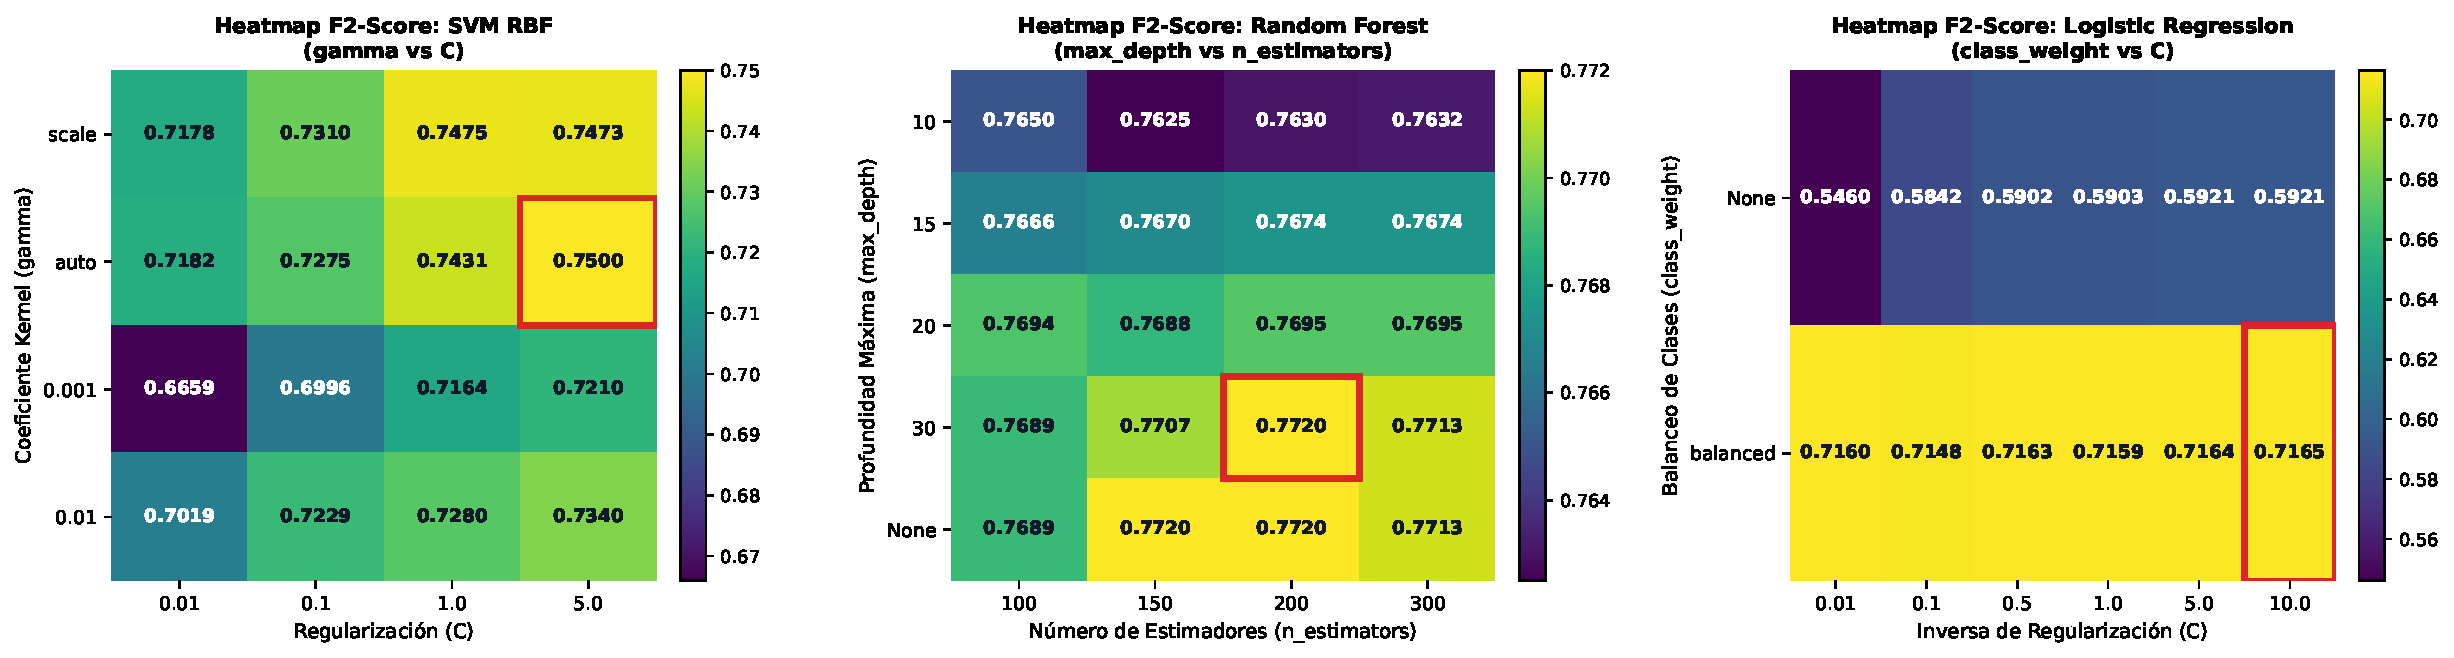
\includegraphics[width=\textwidth]{figures/fig3_tuning_heatmaps.pdf}
\caption{Mapas de calor de validación cruzada 5-fold ($F_2$-Score promedio) sobre $X_{\text{train}}$ para las combinaciones bidimensionales clave manteniendo fijos los restantes hiperparámetros ganadores. El recuadro rojo señala la combinación seleccionada en la Etapa 2.}
\label{fig:tuning_heatmaps}
\end{figure*}

La Fig.~\ref{fig:tuning_heatmaps} expone el comportamiento de la búsqueda de hiperparámetros bajo $F_2$-Score. En \textit{SVM RBF} (con \texttt{class\_weight="balanced"}), incrementar $C$ hacia $5.0$ con \texttt{gamma="auto"} alcanza el máximo $F_2=0.7500$ (frente a $0.6659$ con $C=0.01$ y \texttt{gamma=0.001}). En \textit{Random Forest} (\texttt{min\_samples\_split=10, min\_samples\_leaf=2, max\_features="log2", balanced}), elevar \texttt{max\_depth} de $10$ ($F_2 \approx 0.763$) a $30$ ($F_2=0.7720$) alcanza la meseta óptima junto con \texttt{n\_estimators=200} (compactando el artefacto a $9.46\text{ MB}$). En Regresión Logística se observa un salto claro desde las combinaciones \texttt{None} ($F_2 \le 0.5921$) hacia \texttt{balanced} ($F_2 \approx 0.715$--$0.7165$, óptimo en \texttt{C=10.0}).

\begin{figure*}[t]
\centering
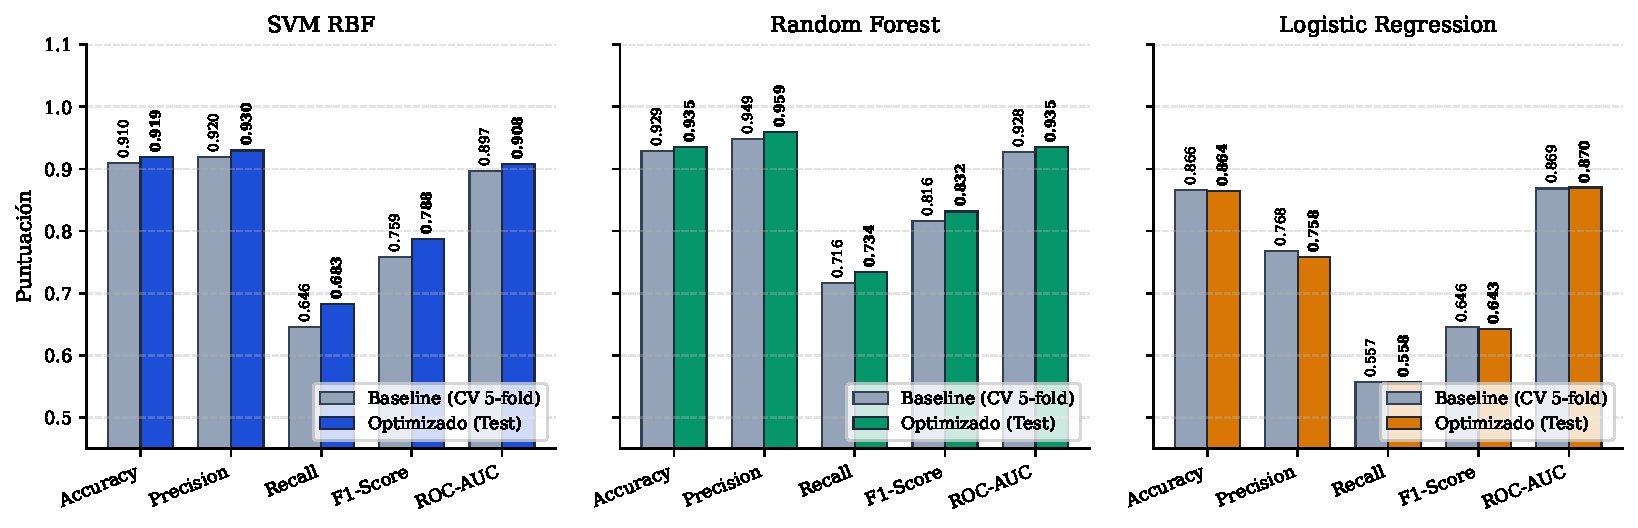
\includegraphics[width=\textwidth]{figures/fig4_baseline_vs_optimized.pdf}
\caption{Comparativa de desempeño entre los modelos base (CV en $X_{\text{train}}$), modelos optimizados por $F_2$ en CV ($X_{\text{train}}$) y evaluación final en el conjunto independiente de prueba ($X_{\text{test}}$, $n=5{,}699$), incluyendo $F_2$-Score.}
\label{fig:baseline_vs_opt}
\end{figure*}

En la Fig.~\ref{fig:baseline_vs_opt} se confirma una generalización consistente hacia $X_{\text{test}}$: los tres modelos optimizados superan sus referentes de CV en exhaustividad, $F_2$-Score y $\text{ROC-AUC}$, preservándose estrictamente la jerarquía $\text{Random Forest} > \text{SVM RBF} > \text{Logistic Regression}$ en todas las métricas compuestas ($F_1$, $F_2$, $\text{ROC-AUC}$ y exactitud).

\begin{figure*}[t]
\centering
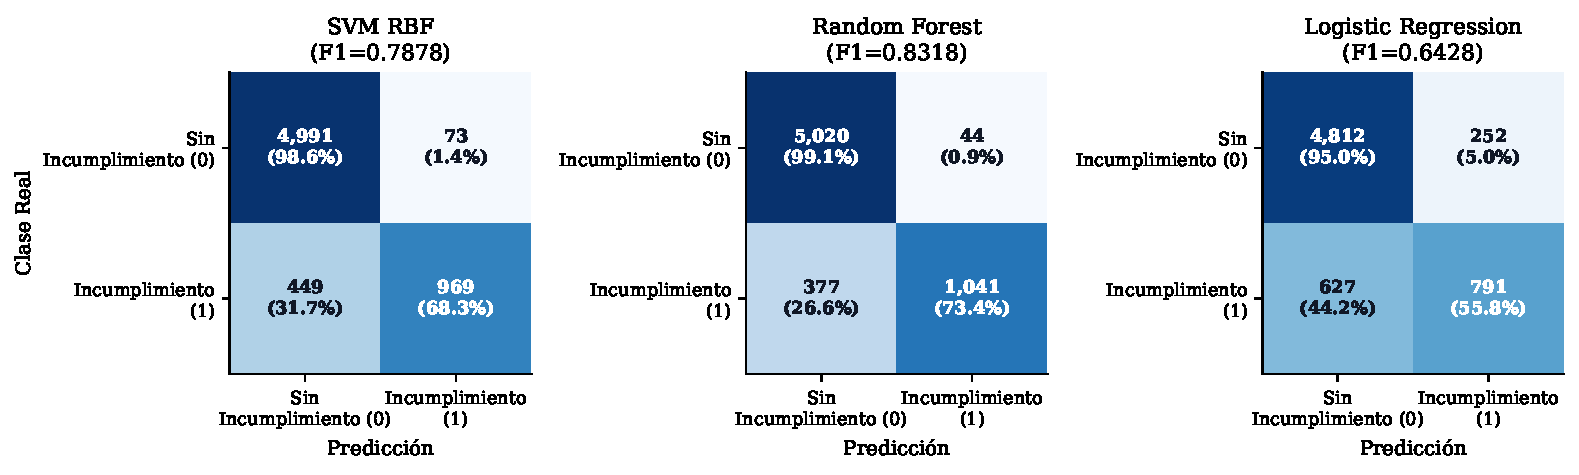
\includegraphics[width=0.96\textwidth]{figures/fig5_confusion_matrices.pdf}
\caption{Matrices de confusión en el conjunto de prueba ($n=5{,}699$: $4{,}462$ sin incumplimiento y $1{,}237$ con incumplimiento) para los modelos optimizados bajo $F_2$-Score, mostrando conteos absolutos, porcentajes por clase real y métricas $F_2$ / $F_1$.}
\label{fig:confusion_matrices}
\end{figure*}

La Fig.~\ref{fig:confusion_matrices} desglosa los aciertos y errores sobre las $5{,}699$ instancias de prueba para los clasificadores optimizados por $F_2$. En la detección de incumplimientos reales (\textbf{Incumplimiento (1)}), \textit{Random Forest} identifica correctamente $977$ de $1{,}237$ casos ($79.0\%$, reduciendo los falsos negativos a $260$), superando a \textit{SVM RBF} ($964$; $77.9\%$, $273$ $FN$) y Regresión Logística ($962$; $77.8\%$, $275$ $FN$). Sin embargo, la diferencia crítica radica en el control de falsos positivos sobre solicitantes solventes (\textbf{Sin Incumplimiento (0)}): \textit{Random Forest} mantiene apenas $199$ falsos positivos ($4.5\%$), frente a $357$ ($8.0\%$) en \textit{SVM RBF} y $764$ ($17.1\%$) en Regresión Logística —reduciendo un $74.0\%$ las falsas alarmas respecto al modelo lineal—.

\begin{figure*}[t]
\centering
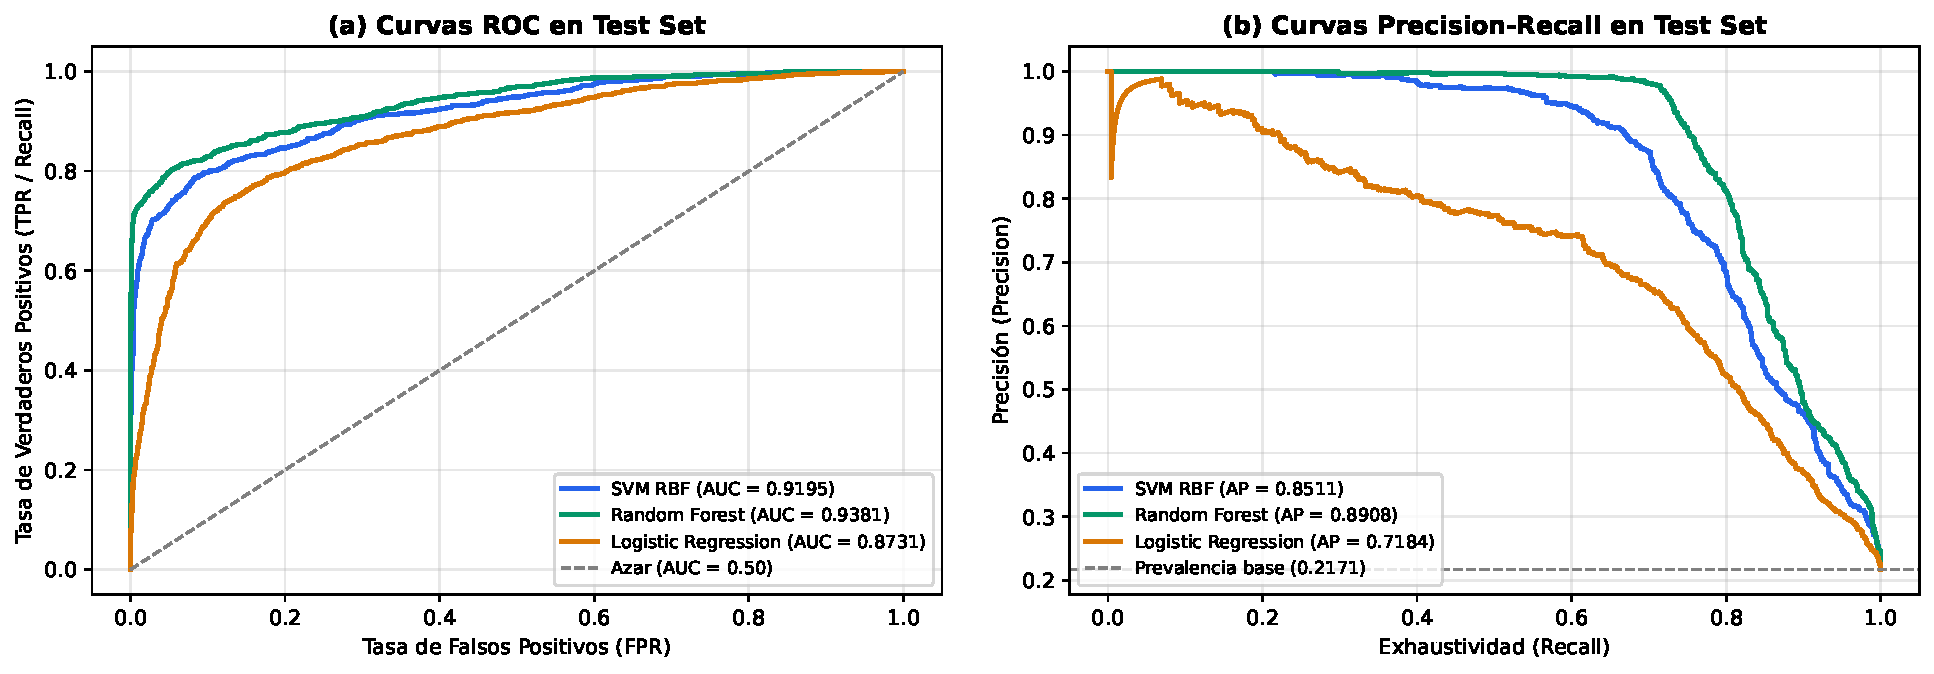
\includegraphics[width=0.95\textwidth]{figures/fig6_roc_pr_curves.pdf}
\caption{Curvas de discriminación probabilística sobre el conjunto independiente de prueba ($n=5{,}699$): (a) curvas ROC con área $\text{ROC-AUC}$; (b) curvas Precision-Recall con área promedio $\text{AP}$ frente a la prevalencia base de $0.2171$.}
\label{fig:roc_pr}
\end{figure*}

Finalmente, la Fig.~\ref{fig:roc_pr} ilustra la separación continua a través de todo el rango de umbrales. En la curva ROC (Fig.~\ref{fig:roc_pr}(a)), \textit{Random Forest} domina el cuadrante superior izquierdo ($\text{ROC-AUC}=0.9381$). En la curva Precision-Recall (Fig.~\ref{fig:roc_pr}(b)) —especialmente exigente ante el $21.71\%$ de prevalencia de incumplimiento—, \textit{Random Forest} alcanza $\text{PR-AUC}=0.8908$ (frente a $0.8511$ de \textit{SVM RBF} y $0.7184$ de Regresión Logística), ofreciendo la mejor capacidad de discriminación para operar a distintos umbrales de riesgo.

\subsection{Discusión de Resultados}

¿Por qué \textit{Random Forest} dominó tan ampliamente tanto en CV como en prueba? La ventaja del bosque aleatorio ($F_2=0.7977$, $F_1=0.8098$, $\text{ROC-AUC}=0.9381$, $\text{PR-AUC}=0.8908$) deriva directamente de la estructura heterogénea del riesgo crediticio en \texttt{credit\_risk\_dataset.csv}. La transición no lineal en \texttt{loan\_grade} (de $20.33\%$ en \texttt{C} a $59.22\%$ en \texttt{D} y $98.31\%$ en \texttt{G}), combinada con umbrales conjuntos en \texttt{loan\_percent\_income}, tipo de vivienda (\texttt{RENT} vs.\ \texttt{OWN}), \texttt{loan\_int\_rate} e historial de mora, genera regiones rectangulares complejas en el espacio de atributos. Mientras la Regresión Logística queda limitada a un único hiperplano global ($F_2=0.7207$, con $764$ falsos positivos al activar \texttt{balanced}) y el núcleo gaussiano de \textit{SVM RBF} sufre en costo computacional al medir distancias isotrópicas sobre $22$ dimensiones ($54.85\text{ s}$), los árboles de \textit{Random Forest} aislan de forma natural las interacciones jerárquicas y mantienen un tiempo de entrenamiento final inferior a un segundo ($0.55\text{ s}$).

Respecto al impacto de la optimización bajo $F_2$, priorizar la exhaustividad $2\times$ sobre la precisión produjo saltos sustanciales frente al \textit{baseline} en los tres modelos ($+0.0483$ en \textit{Random Forest}, $+0.0766$ en \textit{SVM RBF} y $+0.1299$ en Regresión Logística sobre el $F_2$ de prueba), gracias a la adopción unánime de \texttt{class\_weight="balanced"}. Asimismo, las curvas de validación 1D por hiperparámetro en $F_2$ mostraron que combinar \texttt{max\_depth=30} con \texttt{min\_samples\_split=10} y \texttt{min\_samples\_leaf=2} modera la memorización de entrenamiento en \textit{Random Forest} ($F_2$ en fold de entrenamiento $0.9551$ frente a $0.7717$ en validación), conteniendo la varianza. Por su parte, la optimización del umbral de decisión exclusivamente sobre CV en $X_{\text{train}}$ (Tabla~\ref{tab:threshold_cv}) evidenció un margen adicional de hasta $+0.0598$ a $+0.0913$ en \textit{Recall} para escenarios donde minimizar falsos negativos prime sobre la precisión, capacidad integrada de forma interactiva en la aplicación Streamlit sin contaminar la evaluación final en $X_{\text{test}}$.

Entre las limitaciones principales del estudio destacan cuatro aspectos: (i) no se incluyeron algoritmos de \textit{Gradient Boosting} (\textit{XGBoost}, \textit{LightGBM}, \textit{CatBoost}) ni ensambles de apilamiento, los cuales han alcanzado métricas superiores en la literatura reciente~\cite{pucar2026consumer,mahmud2025stacking}; (ii) la evaluación oficial en $X_{\text{test}}$ mantuvo el umbral estándar de $0.50$ para preservar comparabilidad homogénea con la literatura (dejando el umbral CV $F_2$ como opción operativa interactiva en inferencia); (iii) la búsqueda aleatoria de $12$ iteraciones en \textit{Random Forest} cubre solo una muestra del espacio completo, aunque las gráficas 2D confirmaron estabilidad en meseta; y (iv) descartar $3{,}915$ filas incompletas reduce el volumen disponible frente a estrategias de imputación condicional por grupo (\textit{Group-Median} por \texttt{loan\_grade}). Como trabajo futuro se propone integrar \textit{XGBoost} y \textit{LightGBM}, evaluar imputación condicional o \textit{Target Encoding}~\cite{bolikulov2024categorical} y calibrar matrices de costo financiero real para la selección automática de umbrales en producción.

% =========================================================================
\section{Conclusiones}
% =========================================================================

Este trabajo cumplió con el objetivo de diseñar, optimizar y evaluar rigurosamente un flujo reproducible de aprendizaje automático libre de fuga de información orientado a maximizar la detección de incumplimientos crediticios dentro del módulo \texttt{model\_factory}. La depuración determinista previa ($165$ duplicados, $3{,}915$ filas con valores vacíos —preservando el cero numérico— y $6$ atípicos imposibles eliminados sobre $32{,}581$ registros) combinada con la estandarización y codificación encapsuladas dentro de \texttt{Pipeline} y \texttt{ColumnTransformer} garantizó una comparación justa entre Regresión Logística, \textit{SVM RBF} y \textit{Random Forest} sobre una partición estratificada $80/20$ de $28{,}495$ observaciones completas y validación cruzada de $5$ pliegues.

Los resultados experimentales demuestran que \textit{Random Forest} (\texttt{n\_estimators=200}, \texttt{max\_depth=30}, \texttt{min\_samples\_split=10}, \texttt{min\_samples\_leaf=2}, \texttt{max\_features="log2"}, \texttt{class\_weight="balanced"}) ofrece el mejor equilibrio predictivo y eficiencia operativa, alcanzando en el conjunto independiente de prueba una exactitud de $0.9195$, precisión de $0.8308$, exhaustividad de $0.7898$, $F_2=0.7977$, $F_1=0.8098$, $\text{ROC-AUC}=0.9381$ y $\text{PR-AUC}=0.8908$ en solo $0.55\text{ s}$ de entrenamiento final, detectando $977$ de $1{,}237$ incumplimientos con un $74.0\%$ menos falsos positivos que el modelo lineal. \textit{SVM RBF} obtuvo el segundo lugar ($F_2=0.7689$, $F_1=0.7537$, $\text{ROC-AUC}=0.9195$) con un costo computacional $99.7\times$ superior ($54.85\text{ s}$), mientras que Regresión Logística alcanzó alta exhaustividad ($0.7777$) a costa de $764$ falsas alarmas ($\text{Precision}=0.5574$, $F_2=0.7207$).

Adicionalmente, se demostró empíricamente que cuando se prioriza la clase minoritaria ($1$) mediante $F_2$-Score, \texttt{class\_weight="balanced"} resulta consistentemente superior en los tres modelos frente a la ponderación uniforme, y que el ajuste de umbral sobre CV en entrenamiento ($0.37$ en \textit{Random Forest}, $0.21$ en \textit{SVM RBF}) permite elevar el \textit{Recall} por encima de $0.78$--$0.82$ sin fuga hacia prueba. Los modelos serializados en \texttt{models/*.joblib} junto con la aplicación interactiva en Streamlit integran selector dinámico de umbral, análisis por hiperparámetro bajo $F_2$ y auditoría completa para apoyar decisiones de riesgo crediticio.

\bibliographystyle{IEEEtran}
\bibliography{referencias}

\end{document}
